\section{Competing Applications}
\label{sec:competition}

With work and school continuing online, it is even more common to have multiple
applications simultaneously using the home network, potentially leading to
competition between any combination of VCAs, video streaming applications, or other popular
applications. In this section, we measure how VCAs perform in the presence of
other applications sharing the same bottleneck link. We focus on
link sharing with other VCAs, a single TCP flow (iPerf3), and two popular
video streaming applications, Netflix and YouTube (which uses QUIC).


\begin{figure}[t!]
\centering
\begin{subfigure}[t]{.4\textwidth}
    \centering
    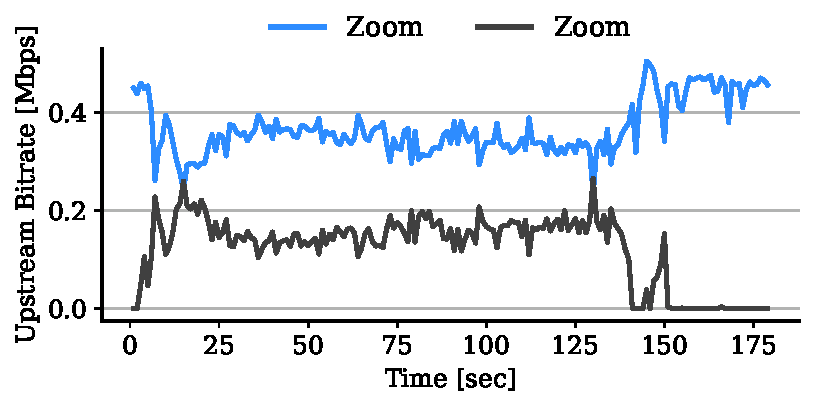
\includegraphics[width=1\textwidth]{figures/comp_ts/zoom_zoom_0.5_ul_r2.pdf}
    \caption{Zoom vs. Zoom}
    \label{subfig:zoom_zoom_0_5}
\end{subfigure}\hfill
\begin{subfigure}[t]{.4\textwidth}
    \centering
    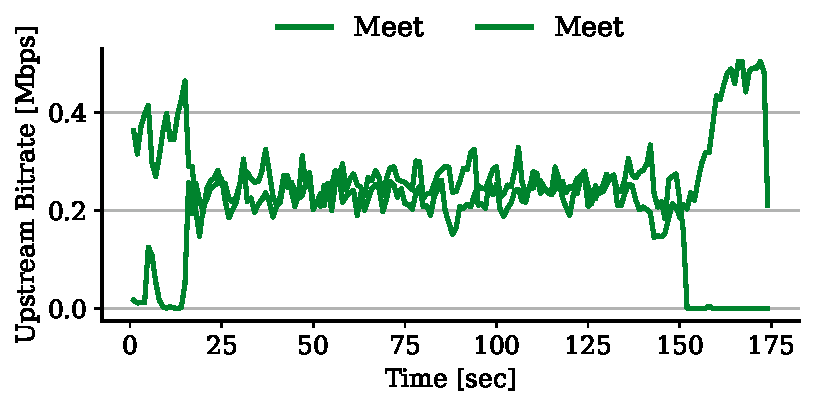
\includegraphics[width=1\textwidth]{figures/comp/meet_meet_0.5_ul_r1.pdf}
    \caption{Meet vs. Meet}
    \label{subfig:meet_meet_0_5}
\end{subfigure}
\caption{Upstream throughput of VCAs in competition on a 0.5~Mbps capacity link. Upper trendline is incumbent application and lower is competing application.}
\label{fig:meet-zoom-upld-0.5}
\end{figure}

\begin{figure*}[t!]
\centering
\begin{subfigure}[t]{.33\textwidth}
    \centering
    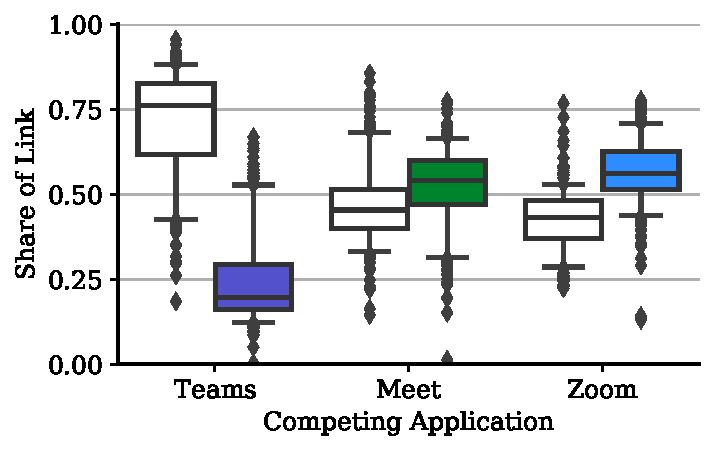
\includegraphics[width=1\textwidth]{figures/comp/box_plot_meet_dl_0.5_all.pdf}
    \caption{Meet}
    \label{fig:meet-dl-boxplot-0.5}
\end{subfigure}\hfill
\begin{subfigure}[t]{.33\textwidth}
    \centering
    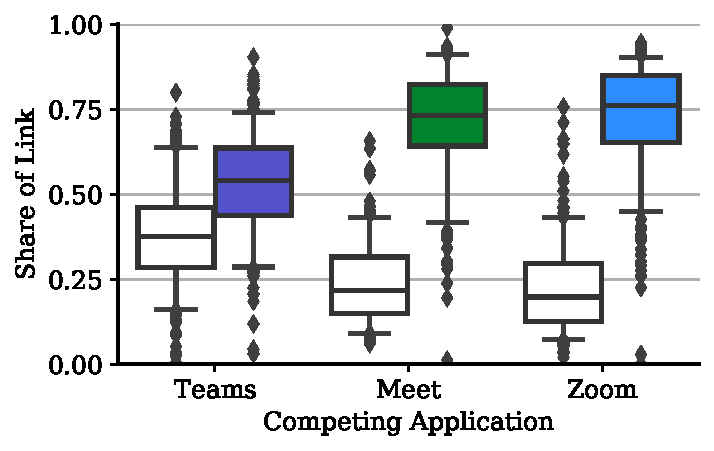
\includegraphics[width=1\textwidth]{figures/comp/box_plot_teams_dl_0.5_all.pdf}
    \caption{Teams}
    \label{fig:teams-dl-boxplot-0.5}
\end{subfigure}
\begin{subfigure}[t]{.33\textwidth}
    \centering
    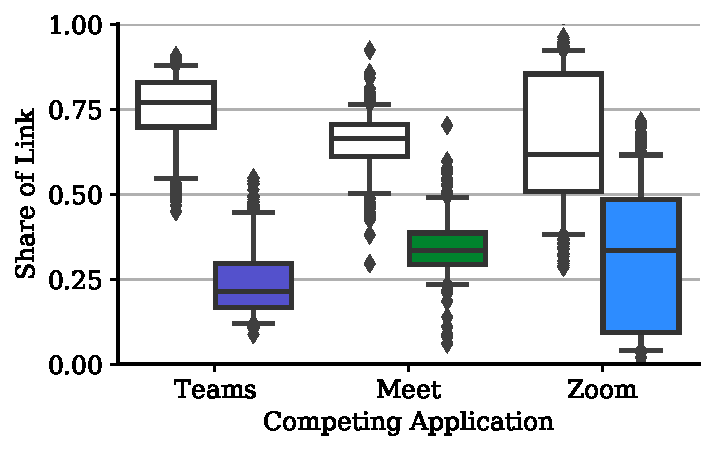
\includegraphics[width=1\textwidth]{figures/comp/box_plot_zoom_dl_0.5_all.pdf}
    \caption{Zoom}
    \label{fig:zoom-dl-boxplot-0.5}
\end{subfigure}
\caption{Downstream bitrate of applications in competition with each VCA on a 0.5~Mbps capacity link.}
\label{fig:dnld-boxplot}
\end{figure*}

\begin{figure}[t!]
\centering
\begin{subfigure}[t]{.5\textwidth}
    \centering
    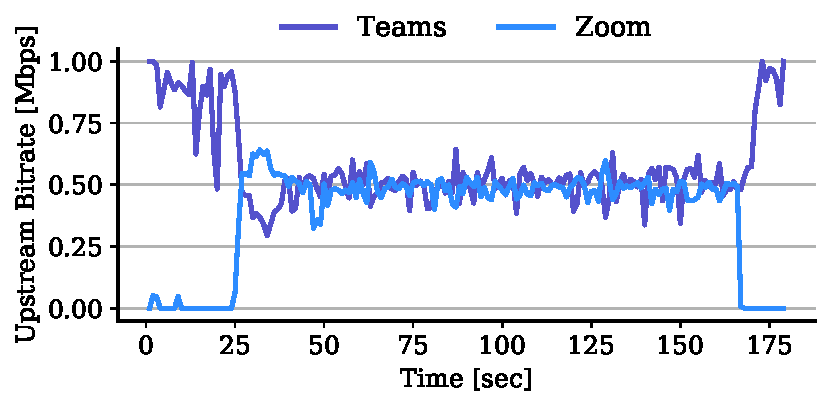
\includegraphics[width=0.8\textwidth]{figures/comp_ts/teams_zoom_1_ul_r2.pdf}
    \caption{Uplink}
    \label{fig:teams-zoom-up-1}
\end{subfigure}\hfill
\begin{subfigure}[t]{.5\textwidth}
    \centering
    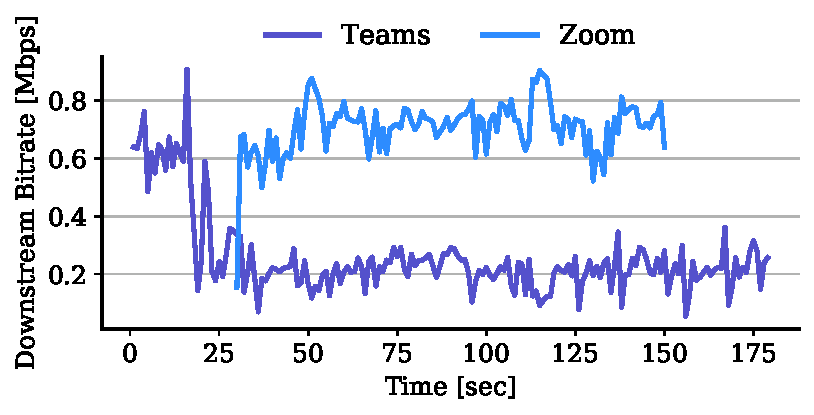
\includegraphics[width=0.8\textwidth]{figures/comp_ts/teams_zoom_1_dl_r2.pdf}
    \caption{Downlink}
    \label{fig:teams-zoom-down-1}
\end{subfigure}
\caption{Comparison of Teams competition behavior in the uplink and downlink}
\label{fig:teams-zoom-1}
\end{figure}


\noindent \textbf{Method}: As illustrated in Figure \ref{fig:competition-setup}, the setup for these experiments differs slightly from earlier ones. 
Instead of connecting the client directly to the router, the two matched clients, C1 and F1, are connected to the router via a switch. 
The link between the switch and the router is shaped by the router. For each test, C1 first establishes a VCA call with C2.
Approximately 30 seconds later, F1 initiates a competing application, which lasts for two minutes.
F1's counter-party, F2, depends on the type of flow.
If the competing flow is a VCA call, then F2 is another consumer laptop.
If the competing flow is an iPerf3\footnote{The iPerf3 server uses TCP CUBIC and is  within the same network (average RTT ~2ms).} (TCP) flow, then F2 is a server on the same network,
  and if the flow is Netflix or Youtube, then F2 is a server for the respective service. Netflix and Youtube are launched directly in Chrome via \texttt{xdg-open}.
After the competing flow terminates, the incumbent flow continues for an additional minute.
We repeat each experiment 3 times, with bandwidth shaped symmetrically at levels of \{0.5, 1, 2, 3, 4, 5\}~Mbps.

\subsection{VCA vs. VCA}


\begin{comment}
We first analyze link sharing between each possible pair of the three VCAs for different shaping level.  

The simplest question is how much bandwidth is required for each VCA to achieve its nominal bitrate, on a shared and constrained link.  Recognizing that the FCC's nominal definition of bandwidth (25/3 Mbps) far exceeds the requirements of multiple VCAs in the downstream direction, we focus on the upstream where the official constraint is less generous.  Figure~\ref{fig:comp_ul} presents the results.  Zoom and Meet plateau around 2~Mbps, while Teams in conjunction with another VCA requires at least 3~Mbps upstream.  Figures for the downstream direction are included in the Appendix, but Meet achieves its nominal performance with a shared link of just 1~Mbps, Zoom, requires 2~Mbps, and within our limited statistics, Teams' downstream consumption does not plateau even at 5 Mbps.

\begin{figure*}
    \centering
    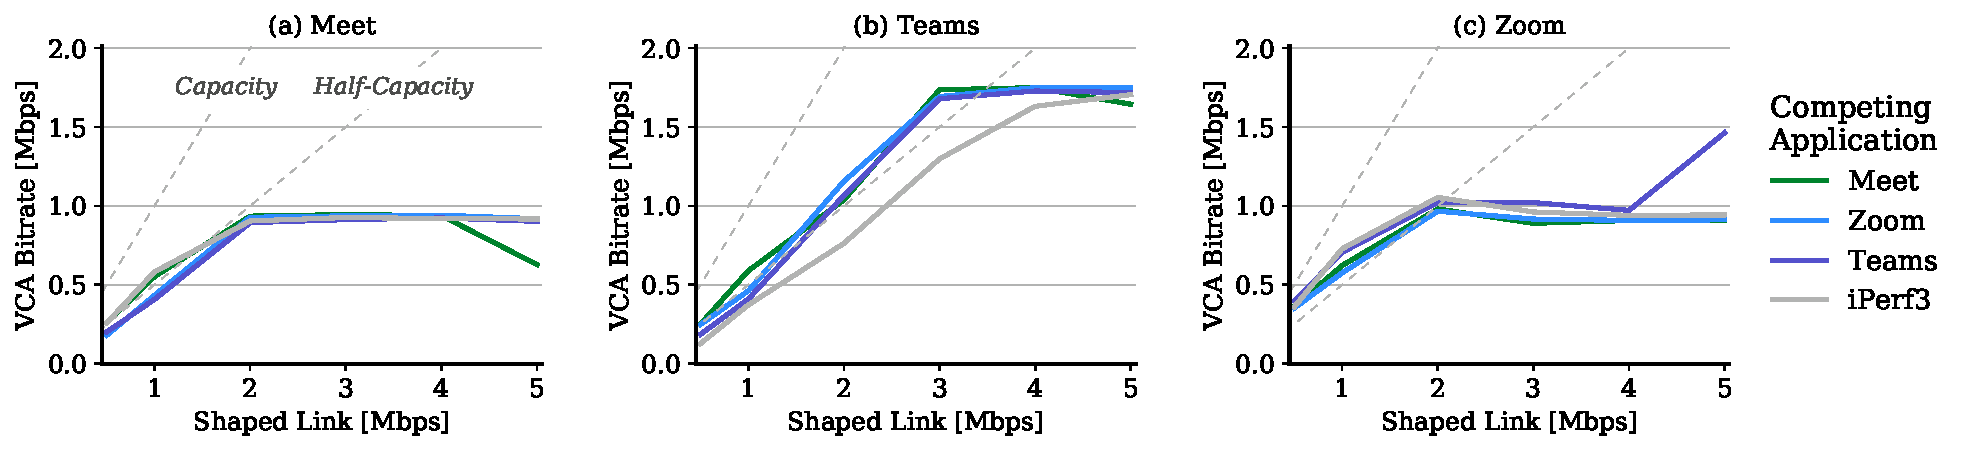
\includegraphics[width=\linewidth]{figures/comp/ul_competition_all.pdf}
    \caption{VCA bitrates on a constrained upstream link, shared with other applications.  Figure labels (a-c) denote the incumbent application, whose bitrates are plotted.}
    \label{fig:comp_ul}
\end{figure*}

Next, we focus on the region with tighter constraints, and competition between the VCAs. Given that there are only two competing clients, we use the proportion of the link shared as a metric to assess fairness. A VCA is termed as aggressive, if it uses more than half of the link capacity under competition, and passive otherwise.
\end{comment}


We find that VCAs are able to achieve their nominal bitrate when the link capacity is 4 Mbps or higher. This is expected as the link capacity exceeds the sum of nominal bitrates of each VCAs. We then focus on the region, when the link capacity is lower, leading to competition between the VCAs. Given that there are only two competing clients, we use the proportion of the link shared as a metric to assess fairness. A VCA is termed as aggressive, if it uses more than half of the link capacity under competition, and passive otherwise.

Looking first at the uplink, we observe differences in how each VCA shares the link. Figure~\ref{fig:boxplot-upld} shows a box plot of the upstream share of an incumbent VCA and a competing VCA when the uplink capacity is 0.5~Mbps.  We find that an incumbent Meet client shares the link fairly with a new Meet or Teams client but backs off when a Zoom client joins (see Figure~\ref{fig:meet_ul_box}). The results are similar for Teams except it receives a slightly higher share while competing with Zoom compared to Meet. Interestingly, Zoom is highly aggressive, both as an incumbent and a competing application, using at least $75\%$ of the link capacity in the case it is an incumbent client (see Figure~\ref{fig:zoom_ul_box}). In fact, Zoom's congestion control is not even fair to itself. Figure~\ref{subfig:zoom_zoom_0_5} illustrates this more clearly with the link sharing between two Zoom clients for a single experiment under 0.5~Mbps uplink capacity. We contrast this with the link sharing between two Meet clients in Figure~\ref{subfig:meet_meet_0_5} where both converge to their fair share of 0.25~Mbps. The results are similar for other uplink capacity with aggressive applications leaving more room for new clients if they achieve their nominal bitrate.  % Clearly, the incumbent Zoom client does not give much room for the   We show the  suggesting that the incumbent Zoom application prioritizes itself regardless of the competing application. 

We find similar results for Zoom and Meet when the downlink is constrained. However, we find that Teams is highly passive in the downlink, backing off to all the VCAs including itself. Figure~\ref{fig:teams-dl-boxplot-0.5} shows the link share of an incumbent Teams client compared to the competing VCA under 0.5~Mbps downlink capacity. Teams is able to utilize only 20\% of the link share with Meet and Zoom. We find similar behavior at other downlink capacities. Figure~\ref{fig:teams-zoom-down-1} illustrates how an incumbent Teams client shares the link with a Zoom client at 1~Mbps downlink capacity. Clearly the Teams client backs off to 0.2~Mbps. This is in contrast to its behavior in the upstream wherein both Teams and Zoom converge to a near fair share of the link (see Figure~\ref{fig:teams-zoom-up-1}). We also notice that the downstream throughput in Figure~\ref{fig:teams-zoom-down-1} for Teams degrades even before the Zoom call starts. This is likely because the competing client opens the Zoom landing page to initiate a call. This can lead to competing TCP traffic on the link and as we find in the next subsection, Teams is highly passive while competing against a TCP flow. % We could not validate this as our traffic capture on the competing device only starts after the call is started.  
% and Teams under  two inconsistencies: i) Meet is more aggressive under constrained downlink Turning to downlink sharing, Meet and Teams no longer consistently behave fairly. Meet consumes over $75\%$ of the downlink bandwidth when competing with Teams. Conversely, Teams backs off when competing with Meet and Zoom. This asymmetrical response is exemplified in Figure X, which compares how Teams competes with Meet on the uplink vs. the downlink. 



% The way each VCA shares the link with other applications is made clear in Figure \ref{fig:dnld-boxplot}. We see that Zoom uses well over $50\%$ of the available capacity against other VCA.

\begin{figure}[t!]
\centering
\begin{subfigure}[t]{.5\textwidth}
    \centering
    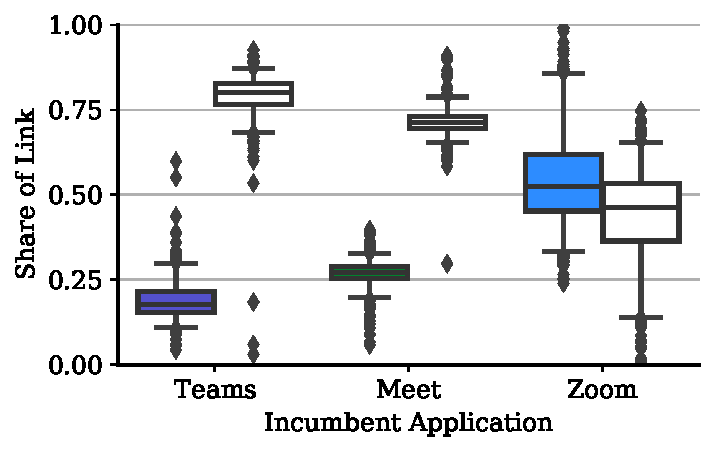
\includegraphics[width=0.7\textwidth]{figures/comp/box_plot_iperf_dl_2.0_all.pdf}
    \caption{Downlink}
    \label{subfig:boxplot-iperf-dl}
\end{subfigure}\hfill
\begin{subfigure}[t]{.5\textwidth}
    \centering
    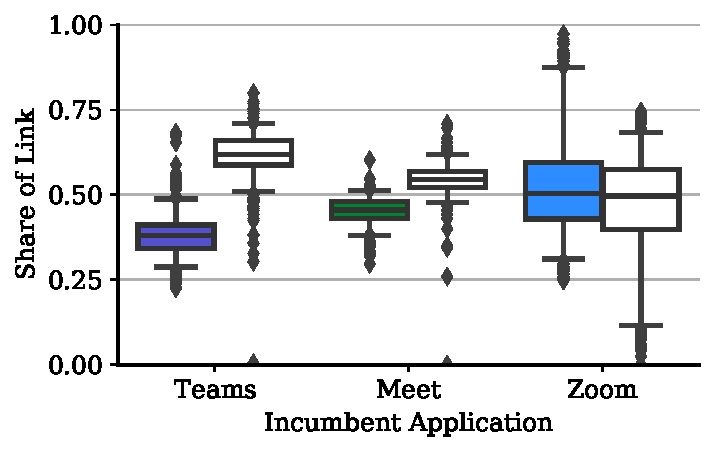
\includegraphics[width=0.7\textwidth]{figures/comp/box_plot_iperfup_ul_2.0_all.pdf}
    \caption{Uplink}
    \label{subfig:boxplot-iperf-ul}
\end{subfigure}
\caption{iPerf3 link sharing with VCAs on a 2~Mbps capacity link.}
\label{fig:boxplot-iperf}
\end{figure}

\begin{figure}[th]
    \centering
    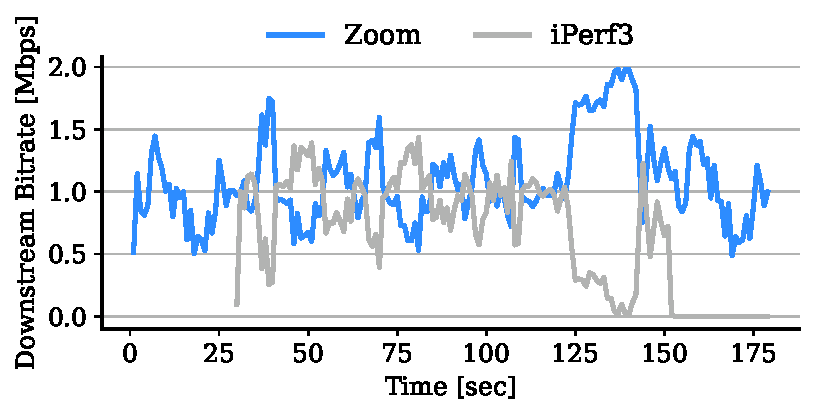
\includegraphics[width=\linewidth]{figures/comp_ts/zoom_iperf_2_dl_r3.pdf}
    \caption{Example of how Zoom probing can adversely affect competing applications}
	\label{fig:zoom-iperf-dl-2}
\end{figure}


\subsection{VCA vs. TCP}

We now compare how the three VCAs compete with a 120 seconds long TCP flow
from iPerf3. In a home network, a long TCP flow can be created by file
download or upload. We find that Zoom is highly aggressive,  especially at low
uplink and downlink capacity, consuming more than 75\% of the bandwidth under
a symmetric 0.5~Mbps link. Meet is TCP-friendly in the uplink direction but
not in the downlink, consuming $75\%$ of the bandwidth at 0.5~Mbps downlink
(figures omitted due to lack of space). Teams, on the other hand, is passive
and backs-off against a TCP flow in both upstream and downstream even at high
link capacity. Figure~\ref{subfig:boxplot-iperf-ul}
and~\ref{subfig:boxplot-iperf-dl} show how each VCA shares a 2~Mbps downlink
and uplink with iPerf3, respectively. Teams is able to use 37\% in uplink and
only 20\% in the downlink even at 2~Mbps. The low upstream throughput for
Teams with a TCP flow is particularly surprising as it was able to achieve its
fair-share when competing against (more aggressive) Meet and Zoom, as shown in Figure~\ref{subfig:teams_ul_box}). Meet and Teams achieve their nominal bitrate allowing iPerf3 to use rest of the link. Clearly, all the VCAs are not TCP CUBIC-friendly with Meet and Zoom being more aggressive and Teams being highly passive. 


\textbf{Anomalous Zoom Bursts}: In the previous section, Figures \ref{fig:ts_upld} and \ref{fig:ts-dnld} showed how Zoom can send bursts of data for an extended period of time following a network disruption. Figure \ref{fig:zoom-iperf-dl-2} shows how this behavior is also exhibited when in competition with iPerf3. At about 125 seconds, Zoom's increased sending rate causes iPerf3 to abruptly lower its utilization. This confirms that the temporary bursts in Zoom, likely for inferring available bandwidth, can adversely affect other applications on a scare link. 


\begin{figure}[t!]
\centering
\begin{subfigure}[t]{.35\textwidth}
    \centering
    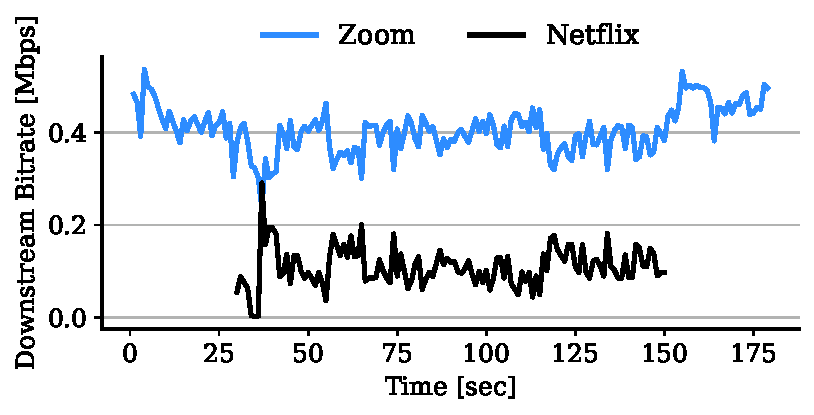
\includegraphics[width=1\textwidth]{figures/comp_ts/zoom_netflix_0.5_dl_r1.pdf}
    \caption{Downstream bitrate for Zoom and Netflix}
    \label{subfig:comp_zoom_netflix_bitrate}
\end{subfigure}\hfill
\begin{subfigure}[t]{.35\textwidth}
    \centering
    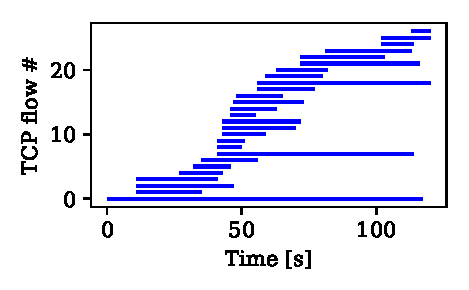
\includegraphics[width=1\textwidth]{figures/comp/netflix_connection_0_5.pdf}
    \caption{TCP connections opened by Netflix}
    \label{subfig:comp_netflix_conn}
\end{subfigure}
\caption{Netflix and Zoom competition on a 0.5~Mbps capacity link.}
\label{fig:comp_netflix_zoom}
\end{figure}
\subsection{VCA vs. Video Streaming}
We also compared VCAs link share against video streaming applications, which are bandwidth intensive downstream. We consider Netflix and YouTube for this analysis. Note that YouTube uses QUIC, a UDP-based transport protocol, which is known to be TCP friendly under some configurations. The goal of this was to understand if there were any differences in VCA's link sharing with applications implemented over TCP or TCP-friendly protocols. We did not find significant deviations from iPerf3 in the downstream. Both Meet and Zoom are highly aggressive, using over $75\%$ of the link capacity while Teams uses less than $25\%$ while competing with YouTube and Netflix at 0.5 Mbps.
We illustrate this in Figure~\ref{subfig:comp_zoom_netflix_bitrate} when a Netflix client competes with an incumbent Zoom client at 0.5 Mbps downlink capacity. Clearly, Zoom achieves an average throughput around 0.4 Mbps while Netflix struggles to reach more than 0.1 Mbps. This is despite Netflix is known to using multiple TCP connections, especially under constrained bandwidth. Figure~\ref{subfig:comp_netflix_conn} shows the TCP connections opened by Netflix during the 120 seconds competition. In total, there are 28 TCP connections with greater than 100 Kbits of data and almost 11 parallel TCP connections at a point. Clearly, It is clear that opening many TCP connections does not improve link sharing for Netflix while competing with Zoom. 

% implementations implemetWe observe similar results when competing with video streaming applications, in which Zoom and Meet consume over $75\%$ of the capacity while Teams uses less than $25\%$. 
% The way each VCA competes with other VCAs is amplified in how they compete with other applications. We did not find significant deviations from iPerf3. Zoom and Meet dominate. Teams backs off. 

% This is particularly interesting because YouTube uses QUIC and Netflix is known to use multiple connections. Prior studies have reported how VCAs. It remains to be seen how application metrics of both the VCA and video streaming application get impacted. 

% Netflix is known to initiate many TCP flows. Figure \ref{subfig:comp_netflix_conn} shows the TCP flows initiated over time by Netflix when in competition with Zoom on a 0.5 Mbps capacity link. 

% Meet and Zoom can command over $75\%$ of the available bandwidth against Netflix, Youtube, while uses under $25\%$. 

\begin{mdframed}[roundcorner=5pt, backgroundcolor=black!10]
\paragraph{Takeaways}: Zoom uses an aggressive congestion control algorithm that dominates the link regardless of whether the competitor is a VCA, one TCP-flow, or multiple TCP-flows. Meet exhibits similar behavior in downlink but is more equitable in uplink. Teams behaves fairly against VCAs on the uplink but backs off in all other cases. 
\end{mdframed}


\begin{comment}

  The notion of fairness between VCAs and video streaming complicates when we consider the link utilization over time. Figure X contrasts the responses of Teams and Zoom to the introduction of a Netflix flow. Looking first at Figure Xa, Teams immediately begins to reduce its consumption once Netflix begins. The available bandwidth is then great enough for Netflix's utilization to reach, allowing it to fill its buffer. Once the buffer is full, Netflix exhibits on-off behavior and Teams recovers/increases its consumption. 

On the other hand, Zoom does not lower its consumption, preventing Netflix from buffering. As a result, both Netflix and Zoom consume at a constant rate throughout the course of the experiment. 
Unlike VCAs, which can not buffer, the average bitrate of video streaming applications can change drastically over time. Figure \ref{fig:ts_zoom_netflix} shows how Netflix and each VCA interact over the course of the experiment. Each interaction is characterized uniquely by a given VCA. \jamie{I would move this up, to part of an `illustration.'}

First, Zoom and Meet do not back off in the presence of Netflix, and continue to receive at the same rate as before. Meet and Zoom both send at a rate lower than $50\%$ of the link capacity. But while Meet and Zoom exhibit similar behavior, their affect on Netflix is different. Because Meet receives at a lower bitrate than Zoom, Netflix maintains a high downlink bitrate as it buffers, before changing to only sporadic bursts of downlink usage. With Zoom, Netflix is not able to buffer, so maintains a constant downlink bitrate. 

Netflix also buffers when competing against Teams. But soon as Netflix is launched, Teams decreases its downlink bitrate, going as low as [insert min bitrate] Mbps. This is both undesirable for VCAs, which are sensitive to changes in bitrate, and an inefficient use of the link. Even in the face of a TCP-based application like Netflix, Teams reduces its downlink consumption. Teams only recovers to its average bitrate once Netflix has finished buffering. 
\end{comment}


% \begin{figure}[t]
%     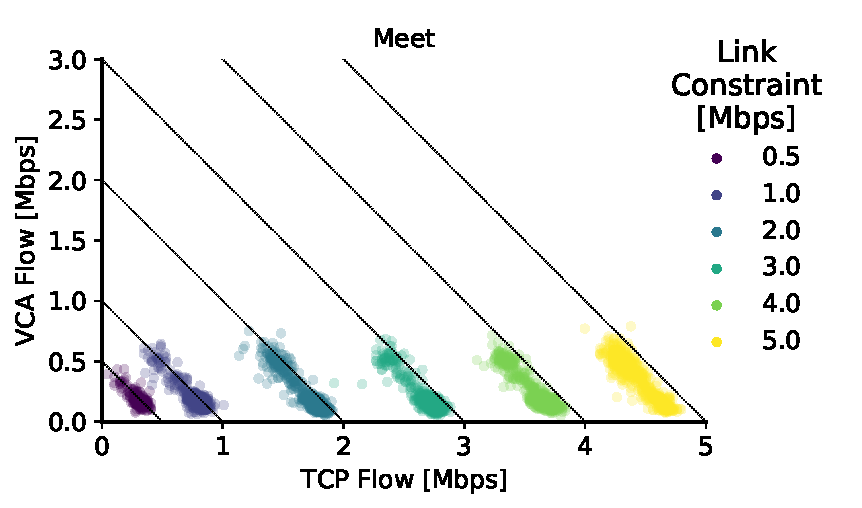
\includegraphics[width=\linewidth]{comp/meet_iperf_scatter.pdf}
%     \caption{Competition between Meet and an iperf3 TCP flow.}
% 	\label{fig:comp_meet_iperf}
% \end{figure}

% \begin{figure}[t]
%     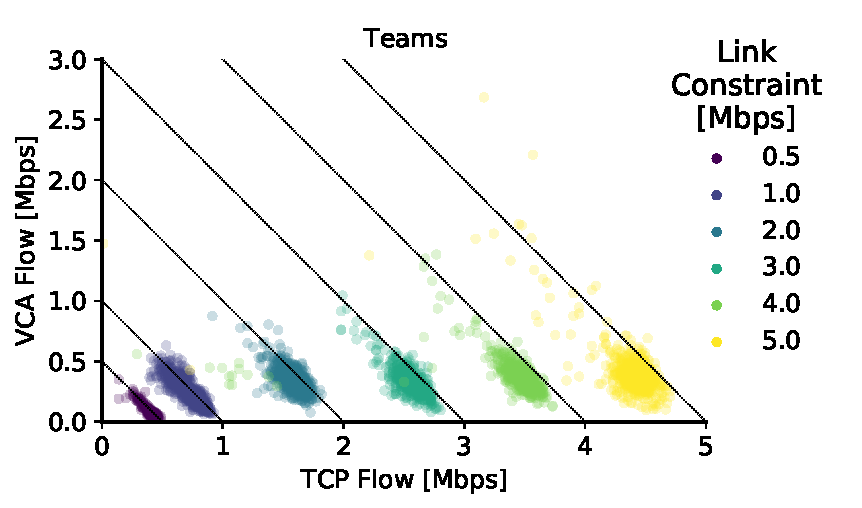
\includegraphics[width=\linewidth]{comp/teams_iperf_scatter.pdf}
%     \caption{Competition between Teams and an iperf3 TCP flow.}
% 	\label{fig:comp_teams_iperf}
% \end{figure}

\begin{comment}
% To study how VCAs compete, the shared link capacity must be less than a threshold defined by each application's nominal bitrate. Using Figure \ref{fig:competition-setup}, let the bottleneck bandwidth be $B$ and C1 and F1's nominal bitrate be $b_1$ and $b_2$, respectively. If $B > b_1 + b_2$, then there is enough bandwidth for both applications to operate at their nominal bitrate. When $B < b_1 + b_2$, the applications must compete over limited bandwidth. We define fairness in competition to be when an application uses half of the available bandwidth. We say that an application is aggressive if it uses more than half and passive if it uses less. 

% When there are simultaneous VCAs on the same network, there will be competition on both the uplink and downlink.


Immediately noticeable is the consistency at which Meet reaches a stable bitrate.%\jamie{awkward} 
Once the link capacity reaches 1~Mbps, Meet's downlink bitrate does not increase with any further link capacity increases. Similarly, Zoom's downlink bitrate peaks at 1 Mbps, which it reaches once the link capacity is 2 Mbps. However, we observe that Teams is far less efficient in sharing the link with competing VCAs. Teams fails to reach a stable downlink bitrate, even when the link is not saturated. In Figure \ref{fig:comp_bitrates_dl}b, we see that Teams has an average downlink bitrate under 1 Mbps when competing against Zoom on a 3 Mbps link. 
We illustrate the basic setup in Figure~\ref{fig:ts_comp_netflix}, 
  pitting the VCAs against Netflix at on a link constrained to 3~Mbps.

From these flows, we construct two variables
  to reflect fairness and performance in the measured flows.
Fairness is represented 
  as the nominal flow's share of two flows constrained link.
In other words, the denominator for the ``share" is
  is the sum of the two flows rather than 
  the shaped link level.
Performance is proxied by bitrate.
Figure~\ref{fig:comp_bitrates_dl}
  displays results for all three VCAs.


Each application uses half the link in ``competition" with itself.
Competition is in evidence primarily at the low end of the domain,
  with the most severe constraints.
Table~\ref{tab:comp} shows the share
  of the flows that each VCA uses,
  at the most-constrained 0.5~Mbps level.
Here, at the low end, Zoom competes
  aggressively and effectively with all other flows:
  it consumes more than three-quarters of the link against Teams, Netflix, and iperf3, 
  and 0.72 against YouTube.
Meet is also quite aggressive at this level, 
  though Zoom ``wins" in direct competition.
Teams fares worse on very-constrained links,
  and does not even compete with the TCP flow.
  


\begin{table}
    \setlength{\tabcolsep}{3pt}
    \fontsize{10.5}{13} \selectfont
    \centering
\begin{tabular}{lcccccc}
\toprule
{} &       Meet &       Teams &        Zoom &     Netflix &     YouTube & iPerf3 \\
\midrule
Meet  &   \cbss{0.47} &  \cbsss{0.74} &   \cbss{0.43} &  \cbsss{0.76} &  \cbsss{0.71} &  \cbsss{0.72} \\
Teams &    \cbs{0.25} &   \cbss{0.41} &    \cbs{0.23} &     \cb{0.17} &    \cbs{0.26} &    \cbs{0.22} \\
Zoom  &  \cbsss{0.66} &  \cbsss{0.76} &  \cbsss{0.68} &  \cbsss{0.75} &  \cbsss{0.73} &  \cbsss{0.72} \\
\bottomrule
\end{tabular}
    \caption{Share of 0.5 Mbps link. Rows are the ``incumbent" VCAs and columns are competing applications.}
    \label{tab:comp}
\end{table}



\end{comment}
